% This LaTeX document is structured to create a comprehensive guide on the ASME 2023 Boiler and Pressure Vessel Code, Section I.
% 
% Document Class:
% - The document class is set to 'article' with 10pt font size and A4 paper size.
%
% Packages Used:
% - inputenc: Allows the use of UTF-8 characters.
% - babel: Sets the document language to Spanish.
% - fontenc: Uses T1 font encoding.
% - lmodern: Uses the Latin Modern font family.
% - microtype: Improves text appearance with micro-typographic extensions.
% - amsmath, amsfonts, amssymb: Provides various mathematical symbols and fonts.
% - authblk: Facilitates the inclusion of author and affiliation information.
% - minted: For syntax highlighting of source code, with 'friendly' style.
% - siunitx: For consistent typesetting of SI units.
% - enumitem: For customizable list environments.
% - graphicx: For including graphics.
% - hyperref: For creating hyperlinks, with customized link colors and back-references.
% - bookmark: For enhanced PDF bookmarks.
% - attachfile: For attaching files to the PDF.
%
% Custom Commands:
% - \@fnsymbol: Redefines the footnote symbol command.
%
% Document Metadata:
% - Title: "Introducción a la sección I 'Reglas para la Construcción de Calderas de Potencia' del código ASME 2023 para calderas y recipientes a presión"
% - Author: Ing. Pablo Barral, with affiliation and contact information.
% - Date: Automatically set to the current date.
%
% PDF Metadata:
% - Configured using \hypersetup for better PDF navigation and metadata.
%
% Document Structure:
% - Includes external files: face.tex, intro.tex, design.tex, sections.tex, annex.tex.
% - Table of contents is generated.
% - Bibliography includes references to ASME codes and relevant literature.

%%%%%%%%%%%%%%%%%%%%%%%%%%%%%%%%%%%%%%%%%%%%%%%%%%%%%%%%
% Paquetes recomendados para mejorar el documento
%%%%%%%%%%%%%%%%%%%%%%%%%%%%%%%%%%%%%%%%%%%%%%%%%%%%%%%%

% --- Estructuración y presentación avanzada ---
% \usepackage{titlesec}       % Personalización avanzada de los títulos de secciones.
% \usepackage{fancyhdr}       % Encabezados y pies de página personalizados.
% \usepackage[a4paper, margin=2.5cm]{geometry} % Configuración de márgenes.
% \usepackage{multicol}       % Documentos con múltiples columnas.
% \usepackage{parskip}        % Ajuste de espacio entre párrafos para mejorar legibilidad.

% --- Tablas y figuras ---
% \usepackage{booktabs}       % Mejor presentación de tablas con líneas horizontales estilizadas.
% \usepackage{caption}        % Personalización de leyendas de figuras y tablas.
% \usepackage{subcaption}     % Subtítulos en figuras o tablas con múltiples subelementos.
% \usepackage{float}          % Control avanzado de la ubicación de figuras/tablas.

% --- Matemáticas y fórmulas ---
% \usepackage{mathtools}      % Extensiones de amsmath para ecuaciones avanzadas.
% \usepackage{cancel}         % Tachar términos en ecuaciones (útil para simplificaciones).
% \usepackage{xfrac}          % Fracciones compactas y estilizadas.

% --- Contenido académico y referencias ---
% \usepackage[backend=biber, style=authoryear]{biblatex} % Gestión avanzada de bibliografía.
% \usepackage{glossaries}     % Creación de glosarios y listas de acrónimos.
% \usepackage{csquotes}       % Manejo avanzado de comillas y citas.
% \usepackage{cleveref}       % Referencias automáticas con nombres contextuales (Figura, Tabla, etc.).

% --- Código y algoritmos ---
% \usepackage{listings}       % Alternativa a minted para incluir código fuente.
% \usepackage{algorithm}      % Presentación de pseudocódigo o algoritmos.
% \usepackage{algpseudocode}  % Complemento para pseudocódigo más avanzado.

% --- Diseño visual y esquemas ---
% \usepackage{tikz}           % Creación de gráficos y diagramas vectoriales.
% \usepackage{pgfplots}       % Generación de gráficos basados en datos.
% \usepackage{xcolor}         % Manejo avanzado de colores.

% --- Elementos adicionales ---
% \usepackage{pdfpages}       % Incluir páginas completas de otros documentos PDF.
% \usepackage{qtree}          % Generación de diagramas de árboles.
% \usepackage{menukeys}       % Representación de combinaciones de teclas o menús.
% \usepackage{tcolorbox}      % Creación de cajas de texto personalizadas.

% --- Accesibilidad y compatibilidad ---
% \usepackage{accessibility}  % Mejora de accesibilidad en documentos PDF.
% \usepackage{polyglossia}    % Soporte avanzado para múltiples idiomas (usar con xelatex o lualatex).

%%%%%%%%%%%%%%%%%%%%%%%%%%%%%%%%%%%%%%%%%%%%%%%%%%%%%%%%
% Fin de las recomendaciones de paquetes
%%%%%%%%%%%%%%%%%%%%%%%%%%%%%%%%%%%%%%%%%%%%%%%%%%%%%%%%




\documentclass[10pt,a4paper]{article}

\usepackage[utf8]{inputenc}
\usepackage[spanish]{babel}
\usepackage[T1]{fontenc}
\usepackage{lmodern}
\usepackage{microtype}

\usepackage{amsmath}
\usepackage{amsfonts}
\usepackage{amssymb}

\usepackage{authblk}

\usepackage[cache=false]{minted}
\usemintedstyle{friendly}
\renewcommand\listingscaption{Código}

\usepackage{siunitx}
\usepackage[shortlabels]{enumitem}


\usepackage{graphicx}

\usepackage[backref=page, colorlinks=true, citecolor=cyan, linkcolor=blue, urlcolor=blue]{hyperref}
\usepackage[numbered]{bookmark}

\usepackage[unicode]{attachfile}


%%% No tocar, generado automáticamente %%%
\makeatletter
\def\@fnsymbol#1{\ensuremath{\ifcase#1\or \dagger\or \ddagger\or
   \mathsection\or \mathparagraph\or \|\or **\or \dagger\dagger
   \or \ddagger\ddagger \else\@ctrerr\fi}}
\makeatother
%%%
     \title{Introducción a la sección I ``Reglas para la Construcción de Calderas de Potencia'' del código ASME 2023 para calderas y recipientes a presión}
     \author{Ing. Pablo Barral\thanks{Departamento de Ing. Mecánica, Universidad de Buenos Aires; 
     \href{mailto:pbarral@fi.uba.ar}{\texttt{pbarral@fi.uba.ar}};
     \raisebox{0.25ex}{\href{https://www.linkedin.com/in/pablo-barral}{
\includegraphics[height=0.75em]{linkedin_logo.png}}}}
     }
     \affil{Sistemas de Almacenamiento}
     \date{\today}

     
     \hypersetup{
          pdfpagemode=UseOutlines,
          pdftitle={Título del Documento},
          pdfauthor={Ing. Pablo Barral},
          pdfsubject={Asunto del Documento},
          pdfkeywords={keyword1, keyword2, keyword3},
          pdfcreator={LaTeX with hyperref},
          pdfproducer={pdfLaTeX}
          pdfstartview=Fit,
          bookmarksnumbered=true,
          bookmarksopen=true,
          bookmarksopenlevel=1,
     }


\begin{document}
     
     \maketitle
     
\begin{abstract}
     Esto es el resumen del texto. %Poner la version que es. Poner para qué materia.\footnote{Poner acá los nombres.}
\end{abstract}

\vspace{1em}
\noindent{\small\textbf{Palabras clave:} ASME, BPVC, calderas}
     \newpage
     \tableofcontents
     \section{Introducción}

La transferencia de calor entre la serpentina y la corriente de aire puede calcularse como

     \begin{equation}
          \dot{Q} = \frac{h_c \cdot A}{c_{p,m}}\cdot\left(h_{sat} - h_a \right)
     \end{equation}

Aquí, $h_{sat}$ es la entalpía del aire húmedo a la temperatura de la serpentina. Esta entalpía es saturada, porque el aire húmedo condensa al tocarla, se genera una película de condensado, por lo que el aire húmedo que está en contacto con esa película se satura. La situación es similar a una torre de enfriamiento.

En este caso, la temperatura del metal es menor que la del punto de rocío del aire. Si ese no fuera el caso, entonces toda la serpentina sería de transferencia de calor sensible, pues no habría forma de que condense. Esta serpentina es la común.

La condensación ocurre antes de que la temperatura promedio del aire húmedo llegue a la temperatura de rocío. Esto es porque el aire húmedo que toma contacto con el metal empieza a condensar mucho antes de que el aire que pasa lejos se enfríe por debajo de su punto de rocío. Hay, en este sentido, un gradiente perpendicular al flujo: gradiente de temperatura y de humedad absoulta.

$h_a$ es la humedad del aire lejos de la serpentina.

Estamos siguiendo las secciones 5.7 y 13.1 del libro de Mitchell. También, unas secciones (SM) aparte.

% Mencionar el ADP y el bypass factor.
% Mencionar la cuenta de una AHU, y hacer un análisis de la energía que se lleva el condensado.


\begin{equation}
     m^{\star}=\frac{\dot{m}_a \cdot c_s}{\dot{m}_w \cdot c_{p,w}}
\end{equation}

cs  es un calor específico efectivo.

Es el cambio de la entalpía con respecto a la temperatura a lo largo de la línea de saturación.

Se evalúa con las temperaturas de entrada y salida.

\begin{equation}
     c_s = \left(\frac{h_{w,sat,in}-h_{w,sat,out}}{T_{w,in}-T_{w,out}}\right)
\end{equation}

Tiene unidades de kJ por C y kg (de aire seco). Es la entalpía del aire húmedo, pero se expresa por unidad de masa de aire seco.

Nos interesa ver la entalpía del aire saturado.

m estrella es como un ratio de calores específicos.

Aa es el área que está expuesta al aire.

eta estrella cero es una eficiencia general para la transferencia de masa, y es un valor cercano a la eficiencia en la transferencia de calor.

hc es el coeficiente convectivo

cpm es el calor específico de la mezcla.

\begin{equation}
     U_0^{\ast}\cdot A_a = \frac{\frac{\eta_0^{\ast}\cdot h_c \cdot A_a}{c_{p,m}}}{1+\frac{c_s\cdot \eta^{\ast}_0 \cdot h_c \cdot A_a}{c_{p,m}\cdot U_w \cdot A_w}}
\end{equation}


\begin{equation}
     {Ntu}^{\ast}=\frac{U_0^{\ast}\cdot A_a}{\dot{m}_a}
\end{equation}

Estaría bueno ver las unidades de lo que estoy escribiendo. Especialmente lo de U asterisco.

\begin{equation}
     \dot{Q}=\dot{\varepsilon}\cdot\dot{m}_a\left(h_{a,in}-h_{w,sat,in}\right)
\end{equation}

El calor, en lugar de hacerlo en función de la temperatura, lo hacemos en función a la entalpía.

Estamos asumiendo que vamos a enfriar, porque hay condensación. Por lo que la entalpía del aire de entrada es mayor a la del agua de enfriamiento.

Si no fuera agua, si fuera refrigerante, el análisis sería similar.

El máximo calor sería cuando el aire esté a la temperatura de entrada del agua.

\begin{equation}
     \varepsilon^{\ast}=\frac{\left(h_{a,in}-h_{a,out}\right)}{\left( h_{a,in}-h_{w,sat,in}\right)}
\end{equation}

\begin{equation}
     \dot{Q}=\dot{m}_w \cdot c_{p,w} \cdot \left(T_{w,out}-T_{w,in}\right)
\end{equation}

   
     \newpage
\section{Diseño}
\subsection{Componentes cilíndricos bajo presión exterior}

El código indica, en el apartado \textbf{PG-27.2.2}, la expresión que debe utilizarse para determinar el espesor mínimo requerido para los caños (\textit{piping}), los domos (\textit{drums}), las envueltas (\textit{shells}) y los colectores (\textit{headers}).

\begin{equation}
     t = \frac{P \cdot D}{2 \cdot S \cdot E + 2 \cdot y \cdot P} + C
     \label{eq:min_req_thickness_od}
\end{equation}

Aquí:
\begin{itemize}
     \item $\mathbf{D}$ es el diametro \underline{exterior} del componente cilíndrico. Una denominación alternativa es $\mathbf{OD}$ (\textit{outside diameter}). 
     
     El diámetro que debe utilizarse es el real, no el nominal. La unidad en que debe expresarse en la ecuación \ref{eq:min_req_thickness_od} es $\SI{}{mm}$.
     
     Por ejemplo, para un caño de $\text{NPS}=\SI{10}{in}$ (\textit{nominal pipe size}), el diámetro nominal es $\text{DN}=\SI{250}{mm}$ mientras que el diámetro exterior es $\text{OD}=\SI{273.1}{mm}$. En este ejemplo, este último es el que debe utilizarse.

     Estos diámetros se establecen en el estándar \textbf{ASME B36.10M}, representando la M al estándar en el sistema métrico.

     \item $\mathbf{P}$ es la máxima presión admisible de trabajo (\textit{MAWP} o \textit{maximum allowable working pressure}). La presión que debe utilizarse, \underline{interna} en este caso, es la \underline{manométrica} o relativa al ambiente, ya que el esfuerzo sobre la pared del componente se genera a partir de la diferencia de fuerzas entre las originadas por la presión absoluta interior y la exterior (la atmosférica).
     
     Su definición se encuentra en el apartado \textbf{PG-21}. La unidad en que debe expresarse en la ecuación \ref{eq:min_req_thickness_od} es $\SI{}{MPa(g)}$.   

     \item $\mathbf{S}$ es la máxima tensión admisible a la tempreatura de diseño del metal. En el apartado \textbf{PG-23} se indica que este valor máximo de tensión admisible puede encontrarse en la \textbf{sección II, parte D, subparte 1, tablas 1A y 1B} del \textbf{BPVC}.
     
     La unidad en que debe expresarse en la ecuación \ref{eq:min_req_thickness_od} es $\SI{}{MPa}$.

     Más detalles pueden encontarse en el apartado \textbf{PG-27.4.2}.

     \item $\mathbf{E}$ es un valor adimensional denominado eficiencia. Más detalles pueden encontarse en el apartado \textbf{PG-27.4.1}.
     \item $\mathbf{y}$ es un coeficiente adimensional de temperatura. Más detalles pueden encontarse en el apartado \textbf{PG-27.4.6}.
     \item $\mathbf{C}$ es un ajuste o margen mínimo para que el componente tenga rigidez estructural (por ejemplo, que no sea sensible a posibles abolladuras por golpes en la manufactura, el transporte, en el caso de que algún operario se pare sobre este), y para tener en cuenta el roscado.
     
     Este margen se suma de manera directa, es un agregado al espesor requerido por el cálculo basado en la presión, el diámetro, la tensión admisible, la eficiencia y el coeficiente de temperatura.

     Más detalles pueden encontarse en el apartado \textbf{PG-27.4.3}.

\end{itemize}

En \textbf{PG-27.4.3} se establece que $C$ no incluyen ningún margen por una posible corrosión o erosión, por lo que este margen debe aplicarse en los casos en que sea necesario.

El código indica, en el mismo apartado, la expresión que debe utilizarse para determinar el espesor mínimo requerido a partir del radio interior (en lugar de determoinarlo respecto del diámetro exterior). Además, incluye las expresiones para determinar la presión interior máxima admisible de trabajo que soportan los componentes a partir de su espesor, tanto para el caso en que se conoce el diámetro exterior como el caso en que se conoce el radio interior.

\subsubsection{Relación con los esfuerzos teóricos}

La ecuación \ref{eq:min_req_thickness_od} puede relacionarse con la expresión de cálculo de la tensión en la dirección circunferencial $\sigma_{\theta}$ (\textit{hoop or circumferential stress}), a veces llamada tensión tangencial, para un cilindro de pared delgada sometido a una presión interior manométrica o relativa al ambiente:

\begin{equation}
     \sigma_{\theta}=\frac{P \cdot d}{2 \cdot t}
     \label{eq:thin_wall_cylinder_int_pressure_01}
\end{equation}

Reagrupando,

\begin{equation}
     t=\frac{P \cdot d}{2 \cdot \sigma_{\theta}}
     \label{eq:thin_wall_cylinder_int_pressure_02}
\end{equation}

La expresión \ref{eq:thin_wall_cylinder_int_pressure_01} se deriva de un equilibro estático de fuerzas entre la inducida por la presión interior (calculada a partir de la superficie proyectada) y la tensión que se genera en el espesor, por lo que aquí $d$ es el diámetro interior. Ver la figura \ref{im:thin_wall_cylinder_int_pressure_01}.

Un recipiente puede considerarse de pared delgada si el diámetro es, al menos, unas 20 veces el diámetro. Por lo tanto, para estos casos, la diferencia entre adoptar $d$ como el diámetro interior o exterior es despreciable.

\begin{figure}[ht]
     \centerline{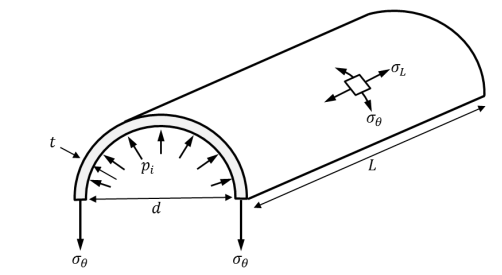
\includegraphics[scale=0.6]{thin_wall_cylinder_int_pressure_01.png}}
     \caption{\textit{Cilindro sometido a una presión interior.}}
     \label{im:thin_wall_cylinder_int_pressure_01}
\end{figure}

\begin{figure}[ht]
     \centerline{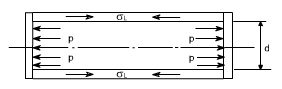
\includegraphics[scale=0.8]{thin_wall_cylinder_int_pressure_02.jpeg}}
     \caption{\textit{Cilindro sometido a una presión interior.}}
     \label{im:thin_wall_cylinder_int_pressure_02}
\end{figure}

La tensión en la dirección longitudinal $\sigma_L$ (\textit{longitudinal stress}), en el caso de que el cilindro tenga tapas, se calcula como

\begin{equation}
     \sigma_L=\frac{P \cdot d}{4 \cdot t}
     \label{eq:thin_wall_cylinder_int_pressure_03}
\end{equation}

La expresión \ref{eq:thin_wall_cylinder_int_pressure_03} se deriva de un equilibro estático de fuerzas entre la inducida por la presión interior (calculada a partir de la superficie proyectada) y la tensión que se genera en el espesor, por lo que aquí $d$ es el diámetro interior. Ver la figura \ref{im:thin_wall_cylinder_int_pressure_02}.

Para un recipiente de pared delgada, la tensión en la dirección radial $\sigma_{r}$ (\textit{radial stress}) es mucho menor que las otras dos tensiones, y puede desestimarse. Por lo tanto, el sistema conforma un estado plano de tensiones perpendiculares entre sí, siendo $\sigma_{\theta}$ y $\sigma_L$ las tensiones principales de ese sistema.

\paragraph{Nota importante:} Si bien las ecuaciones \ref{eq:min_req_thickness_od} y \ref{eq:thin_wall_cylinder_int_pressure_01} están relacionadas, la que debe utilizarse al diseñar según el código es \ref{eq:min_req_thickness_od}, ya que esta contiene las características del material y sus propiedades, los efectos de la merma de resistencia del material por el efecto de la temperatura de diseño, la adopción de un coeficiente de seguridad, el debilitamientos en el caso de que el cilindro esté agujereado, el debilitamiento por las costuras de la soldadura, la adopción de un margen para una resistencia estructural propia ante golpes o abolladuras, el efecto del estado plano de tensiones, etc. 

\subsubsection{Ejemplo de cálculo}

Supongamos que se quiere dimensionar el espesor del domo de una caldera acuotubular. Consideremos una $\text{MAWP}=\SI{75}{bar(g)}$, una temperatura de diseño $T=\SI{290}{\celsius}$, que el diámetro exterior es $D=\SI{69,5}{in}=\SI{1765.3}{mm}$ que el material es SA-516 Gr. 70 y, únicamente para los fines de este ejemplo, que el domo no posee costuras de soldadura.

Determinando la eficiencia, el coeficiente de temperatura, la máxima tensión admisible a la temperatura de diseño del metal y considerando que no debe adicionarse el margen $C$, al reemplazar en \ref{eq:min_req_thickness_od}, resulta

\begin{gather*}
     t=\frac{\SI{7,5}{MPa(g)}\cdot\SI{1765,3}{mm}}{2\cdot\SI{137,6}{MPa}\cdot 1,0+2\cdot 0,4\cdot \SI{7,5}{MPa(g)}}\\
     \boxed{t=\SI{47,08}{mm}}
\end{gather*}

\subsection{Material}

Acá quiero mostrar:

\begin{enumerate}
     \item La limitación de que el material tiene que estar en ASME II. PG-5.
     \item Para chapa (plate), veo PG-6.
     \item Para el ejemplo, dar las características del acero que utilizo. Sus valores de resistencia mecánica, las notas que lo rigen, el gráfico que hice, el valor de resistencia mecánica. ASME Parte 2
     \item Los apéndices no mandatorios del código ASME II sobre grafitización.
     \item La composición y el estándar ASTM que me rige. Esta en ASME II Parte A.
\end{enumerate}

\begin{figure}[ht]
     \centerline{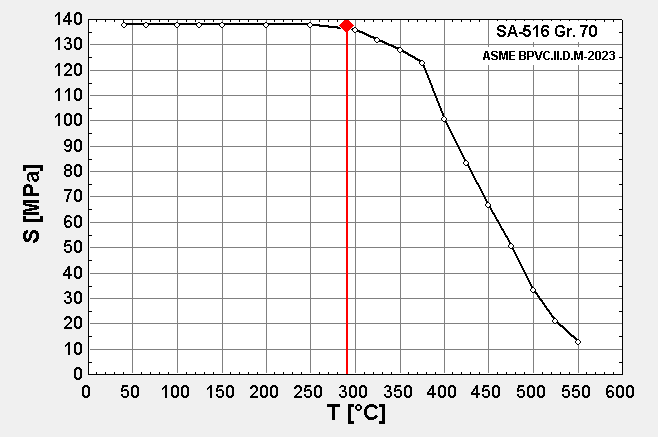
\includegraphics[scale=0.6]{mat_prop_example_01.png}}
     \caption{\textit{TBD.}}
     \label{im:mat_prop_example_01}
\end{figure}


\begin{table}[!ht]
     \centering
     \begin{tabular}{cc}
         \hline
         Columna 1 & Columna 2 \\
         \hline
         Fila 1, Col 1 & Fila 1, Col 2 \\
         \hline
         Fila 2, Col 1 & Fila 2, Col 2 \\
         \hline
         Fila 3, Col 1 & Fila 3, Col 2 \\
         \hline
         Fila 4, Col 1 & Fila 4, Col 2 \\
         \hline
         Fila 5, Col 1 & Fila 5, Col 2 \\
         \hline
         Fila 6, Col 1 & Fila 6, Col 2 \\
         \hline
     \end{tabular}
     \caption{Ejemplo de tabla con dos columnas y seis filas}
     \label{tabla:ejemplo}
 \end{table}

\subsection{MAWP}

\subsection{Temperatura de diseño}

\subsection{Tensión admisible}

\subsection{Eficiencia}

\subsection{Coeficiente de temperatura}

\begin{enumerate}
     \item Acá voy a poner la temperatura de diseñp
\end{enumerate}










%PAGINA 20 tabla 1A

%linea 45

%resistencia mecanica minima 485 MPa
%fluencia minima 260 MPa
%G10 S1 T2
%Limite maximo de temperartura 454 C

%buscar si tengo algun calculo ferrer de estos
%tiene soldaduras longitudinales y cirfunferenciales

%cabezal de medida distinta a la envueltas
%Ver PG-6, que me admite este material
%considerando que domo va aislado, lo vamos a poner todo a temperatura de saturacion

%apendice de grafitizacion

%asme II non mandatorio A 201 y 202

%mencionar algo de la eficiencia de la soldadura. Medio que pasarlo por alto, la verdad.

%Lo mismo sobre los casquetes, para no marearme yo y no marear a los estudianbtes.

%Sí poner lo de la grafitizacion.







     \newpage
\section{Ligamentos}

Acá tengo que poner los casos simples y algunos de los casos complejos.

Ver cuando haga ese mini ejercicio para que entreguen, qué quiero poner, como para que tengan algo de variedad.



PG-52 estamos hablando.




%% ver si VPI me presentó un reporte según ASME I.
%% ademas de los ligamentos y las aperturas, ver si menciono algo de los dished heads

%% en cuanto a los desaireadores, poner los tipo de relleno, ver el perry, ver los eductores, ver que estan elevados, ver las toberas, ver el venteo arriba, ver desde el proceso por qué los tengo.

%% ver relleno empaquetados, placas.

%% ASME VIII Div. 1 Ver si VPI me reporto algo de este tacho, incluso lo puedo motrar en clase.

%% Podría llegar a mencionar un tanque flash como otro tanque dentro del alcance de la caldera, y del tanque de enfriamiento de purgas, que si bien tiene una presión mínima, le viene la purga presurizada.

%% Y obviamente, todos los colectores intermedios de caldera, y el colector de vapor sobrecalentado. Todo esto tiene uqe analizarse según código.

%% Se puede estampar el diseño, la fabricación y el montaje. Estampa parcial creo que refiere a los primeros dos.
%% Estampa completa, incluyendo el montaje, es sustantivamente caro si es que tengo que contratar al inspector. Chequear esto, por las dudas


%% bajar el perry novena edicion de libgen en la uba no me deja

\newpage
\section{Derivaciones y compensaciones}

PG-32

Como recomendación de diseño es dable pensar que no vamos a poner los cordones de soldadura, como hace Sobral.

Mandárselo para que le pegue una mirada.












\newpage
\section{Válvulas de seguridad}

Entre los apartados \textbf{PG-67} y \textbf{PG-73}, el código se dedica a establecer los requerimientos para los dispositivos de protección contra la sobrepresión\footnote{Se sobreentiende que la sobrepresión se refiere a un valor por encima de la \textit{MAWP}. Más detalles se presentan más adelante.}.\footnote{El código utiliza la denominación de válvula de alivio de presión (\textit{pressure relief valves}) de manera general, sin entrar en ninguna distinción con la denominación de válvula de seguridad (\textit{pressure safety valve}).} %Es importante destacar que la sección I del código no brinda herramientas para dimensionar los dispositivos de alivio de presión. En lugar de eso, simplemente establece los requerimientos que debe cumplir.

El código genera requerimientos para lo que llama caldera (\textit{boiler}) en el apartado \textbf{PG-67} y para los sobrecalentadores y recalentadores en \textbf{PG-68}. Los requerimientos para los dispositivos de alivio de presión para los economizadores (en los casos en los que apliquen) se encuentran también en el apartado \textbf{PG-67}. La denominación de ''caldera´´ que aquí se usa debe entenderse como la parte del equipo en donde se genera vapor (sea el hogar, sean los tubos pantalla o el haz convectivo si los hubiere).

\subsection{Calderas}

El primer requerimiento que genera el código (en el apartado \textbf{PG-67.1}) es que todas las calderas tienen que tener por lo menos una válvula de alivio de presión. Más aún: las calderas de tubos lisos/desnudos (\textit{bare tubes}), es decir, sin la superficie extendida generada por las aletas, cuya superficie calefactora supere los $A=\SI{47}{m^2}$ deben tener, por lo menos, dos válvulas de alivio de presión. Cuando la superficie calefactora se logra con tubos aletados, el requerimiento de contar con al menos dos válvulas de seguridad se indica para calderas cuya máxima generación de vapor de diseño (establecida por el fabricante) supere $G=\SI{1800}{kg/h}$. Esto es porque la superficie extendida se utiliza con fuentes térmicas de bajo nivel, por lo que puede haber diseños con temperarturas bajas, mucha superficie calefactora y poca generación de vapor para los que el requerimiento de dos válvulas por lo menos es demasiado estricto.

El segundo requerimiento es sobre la capacidad del conjunto de válvulas y sobre el set\footnote{Algunas denominaciones comunes son: timbre, tarado de la válvula, punto de disparo.} de cada una de ellas. Esto es: el punto en el que se inicia la apertura.

El código requiere en el apartado \textbf{PG-67.2.1} que la capacidad de descarga, de alivio (\textit{relieveng capacity}), combinada entre todas las válvulas, sea equivalente a todo el caudal de vapor que puede generar la caldera para todos sus combustibles y de acuerdo con su sistema de combustión, \textit{cuando la caldera está a la $\mathbf{MAWP}$}. Este es un valor que debe informar el fabricante, y puede ser superior que el caudal generable de diseño (\textit{MCR o maximum continuous rating}), debido a los márgenes con los que se diseña la caldera.\footnote{El código presenta algunas sutilezas más en el apartado \textbf{PG-67.2.1} acerca de la capacidad de descarga de las válvulas. Estas reglas debe tenerse en cuenta para el diseño. En \cite{MacKay_Pillow} se encuentra una explicación acerca de esto.}

Naturalmente, una válvula (que no es otra cosa que un orificio calibrado) chica necesita más presión interna para poder descargar ese caudal de vapor que una más grande. Por otra parte, es esperable que la presión crezca mientras la válvula comienza a actuar y hasta que llegue a su capacidad máxima de descarga, ya que estas no actúan inmediatamente.

Para dar cuenta de esto, el código requiere en el apartado \textbf{PG-67.2} que la presión en el interior de la caldera cuando se descarga al exterior toda la capacidad de generación de vapor no supere el 6\% del mayor valor de set de las válvulas. Y, además, que esta presión no supere el 6\% de la $\mathbf{MAWP}$.

Supongamos como ejemplo que una caldera tiene dos válvulas: una con set de $\SI{95}{bar(g)}$ y otra de $\SI{100}{bar(g)}$. Es decir: la primera comienza a abrir cuando la presión interna supera los $\SI{95}{bar(g)}$, y la segunda cuando se superan los $\SI{100}{bar(g)}$. El código requiere que la capacidad total combinada de descarga sea alcanzable cuando la presión interior sea $\SI{106}{bar(g)}$ (como máximo). Este valor debe ser menor que el 106\% de la $\mathbf{MAWP}$.

Esto no implica necesariamente que la $\mathbf{MAWP}$ sea mayor que todos los valores de set de las válvulas. Podría suceder que fuera menor que alguno. En el ejemplo, si la capacidad de descarga total se lograse en $\SI{102}{bar(g)}$ (es decir: permitiendo sólo un 2\% -menor al 6\% máximo- de incremento de presión para la válvula que abre última), podría darse el valor $MAWP=\SI{95}{bar(g)}$. 

En el apartado \textbf{PG-67.2}

Cabe recordar aquí que el código requiere que cualquier presión operativa, permanente o transitoria, no debe superar la $\mathbf{MAWP}$, y que el uso de los dispositivos de alivio es únicamente para situaciones imprevistas.



% poner el dimensionamiento. Poner algun ejemplo. Poner formula. Pensar en que puedan calcular.
% poner eso del 3%
% poner que hay requerimientos sobre el sobrecalentador y sobre el economizador
% hablar de las imagenes que elegi
% aclarar que en la seccion IV I VIII y API son todos requerimientos distintos
% poner en la bibliografia los apuntes que me gusten, y poner el codigo seccion XIII
% Si no pongo mucho más sobre sobrecalentadores y economizadores, borrar la subseccion y dejar solo la seccion










% sobre el dimensionamiento, esta 9764, ahi esta la formula, la tabla para Ksh esta en ASME I. ASME I refiere a ASME XIII, segun interpreto, hay un KD que tiene dar el fabricante (ensayado). Con eso se dimensionan.

% esta libro es una excelente guia y lo explica perfecto
%The Safety Relief Valve
%Handbook
%%Design and Use of Process Safety
%Valves to ASME and International
%Codes and Standards
%Marc Hellemans

%ponerlo en la bibliografia.
% Con esto damos una idea del dimensionamiento.

% Buscar Ksh en el codigo ASME I
% Poner ASME XIII en la bibliografia.

% poner que hay diferencias entre API 520 y ASME VIII. No entraremos en detalles, pero hay diferencias.

% KD es ese coeficiente de descarga, es el que es entre teorico y ensayado, real


 % creo que no interprete bien lo del set, creo que peude ir mas del 6%.

 %Pressure relief valve
%%engineering handbook
%Anderson Greenwood, Crosby And VAreC produCts | Technical publicaTion no. Tp-V300

%de emerson, tiene ejemplos de calculo

%El "simmer" es una apertura gradual y parcial de la válvula antes de alcanzar la presión de ajuste.
%El "popping" es la apertura completa y repentina de la válvula cuando se alcanza la presión de ajuste.

%chatter

%blodown, que es la presio nde reset
%luego, el drain de la descarga

% conservar estas notas aqui, no borrarlas

% K = 0.9 x Kd

% ahi lo dice 9.7.6.5

% ver cómo citar la bibliografía.






















%chequear el libro de mckay, a ver qué dice más lo de psvs que baje
% en principio la formula no la voy a poner.
% Tratar de hacer un resumen, aunque voy a tener que leer un poquito sobre esto.
% poner en la bibliografia algo de calculo de las PSVs, lo que me baje
% el de mckay lo explica bien, leerlo y robar data de alli.

% ALGO IMPORANTE ES QUE EL CODIGO ASME I NO DICE COMO DIMENSIONAR LA VALVULA, SOLAMENTE LE IMPONE REQUERIMIENTOS


% https://annas-archive.org/md5/f922373c882e21d6952f62544dd74d06

% https://annas-archive.org/md5/106071f4ddefd408f383586cd2bd54dd

% https://annas-archive.org/md5/d8c268ec7a4e4c53d73fd806f94a3b74


%PG-67.1
%Minimum Number of Pressure Relief Valves Required

%Dbe have two or more pressure relief valves

%Los dispositivos de alivio de presión son las PSV, pressure safety valve, las válvulas de seguridad, coloquialmente.


%PG-67.2
%The total combined relieving capacity for
%each boiler (except as noted in PG-67.2.1.6, PG-67.4,
%and PL-54) shall be such that all the steam that can be
%generated by the boiler is discharged without allowing
%the pressure to rise more than 6\% above the highest

%Acá se completa lo que vimos en la MAWP. No sólo la sobrepresión admisible cuando se están descargando, sino qué caudal deben descargar. Con esto, se pueden dimensionar los dispositivos.

%PG-67.3
%One or more pressure relief valves on the
%%boiler proper shall be set at or below the maximum allow-
%able working pressure (except as noted in PG-67.4). If
%additional valves are used the highest pressure setting
%shall not exceed the maximum allowable working pres-
%sure by more than 3\%. The complete range of pressure
%%settings of all the saturated-steam pressure relief valves
%on a boiler shall not exceed 10\% of the highest pressure to
%%which any valve is set. Pressure setting of pressure relief
%valves on high-temperature water boilers15 may exceed
%this 10\% range. Economizer pressure relief devices
%required by PG-67.2.1.6 shall be set as above using the
%MAWP of the economizer


%Poner una foto de una válvula de seguridad, que se vea el resorte ,el tornillo de calibracion, y una foto en la que se vean en una caldera, tanto en una humo como en el domo.

%Chequear pero creo que tanto el eco como el sobrecalentador o el recalentador deben tener sus propios dispositivos de alivio.

%chequear si si  si tienen que ser dos

\begin{figure}[ht]
    \centerline{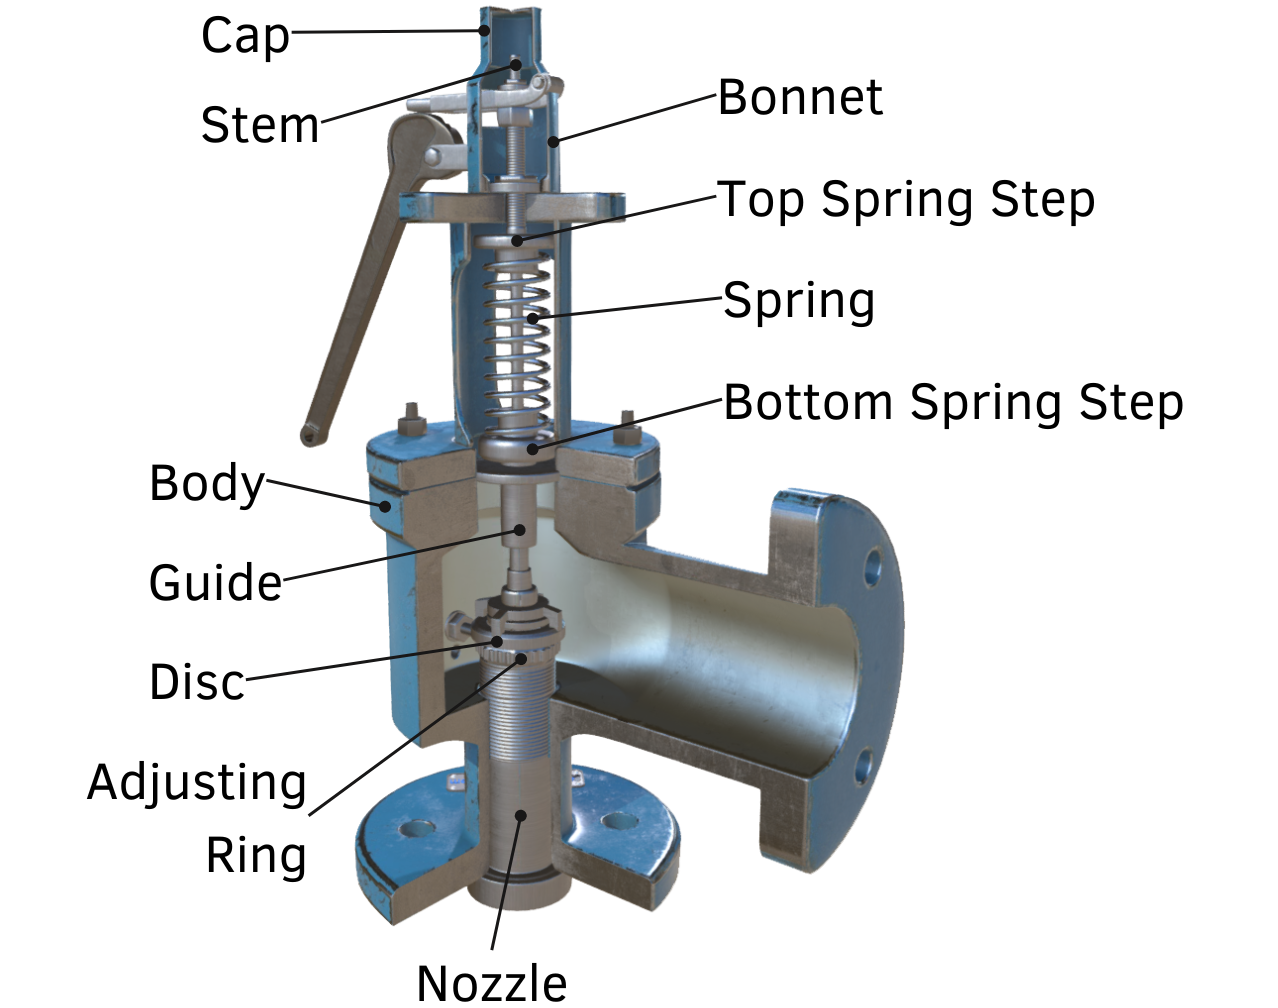
\includegraphics[scale=0.2]{spring_loaded_safety_valve_01.png}}
    \caption{\textit{TBD.}}
    \label{im:spring_loaded_safety_valve_01}
\end{figure}

\begin{figure}[ht]
    \centerline{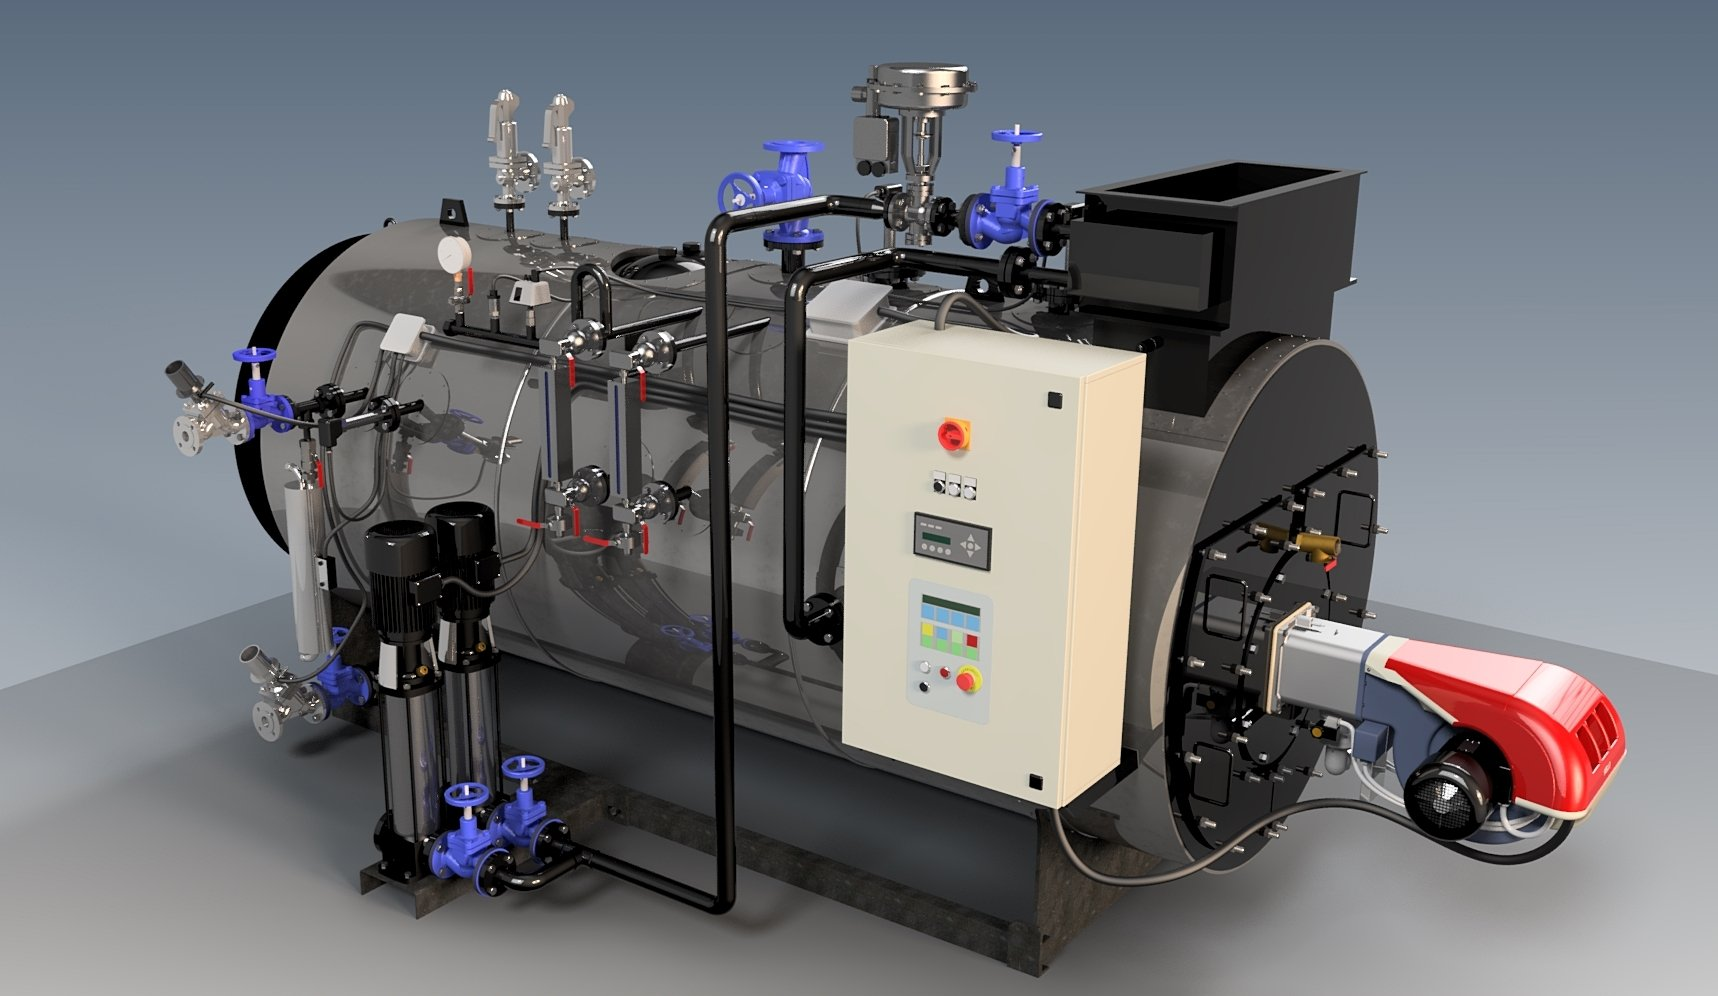
\includegraphics[scale=0.2]{two_psv_firetube_boiler.jpg}}
    \caption{\textit{TBD.}}
    \label{im:two_psv_firetube_boiler}
\end{figure}





\newpage
\section{Comentarios finales y conclusiones}

Poner aca todo lo que dejamos por afuera, o mencionar algunas de las partes.

Concluir algo.








%PAGINA 20 tabla 1A

%linea 45

%resistencia mecanica minima 485 MPa
%fluencia minima 260 MPa
%G10 S1 T2
%Limite maximo de temperartura 454 C

%buscar si tengo algun calculo ferrer de estos
%tiene soldaduras longitudinales y cirfunferenciales

%cabezal de medida distinta a la envueltas
%Ver PG-6, que me admite este material
%considerando que domo va aislado, lo vamos a poner todo a temperatura de saturacion

%apendice de grafitizacion

%asme II non mandatorio A 201 y 202

%mencionar algo de la eficiencia de la soldadura. Medio que pasarlo por alto, la verdad.

%Lo mismo sobre los casquetes, para no marearme yo y no marear a los estudianbtes.

%Sí poner lo de la grafitizacion.







     \section{Anexo}
\inputminted[frame=lines, framesep=2mm,fontsize=\footnotesize,linenos]{python}{code_02.py}    


     
     \newpage
     \begin{thebibliography}{9}
          \bibitem{BPVC.I-2023}
          ASME (2023), \emph{Boiler and Pressure Vessel Code (An International Code) - Section I ``Rules for Construction of Power Boilers''}, ASME.
          \bibitem{BPVC.II.A-2023}
          ASME (2023), \emph{Boiler and Pressure Vessel Code (An International Code) - Section II ``Materials'' - Part A "Ferrous Material Specifications" - Volume 1 \& 2}, ASME.
          \bibitem{BPVC.II.D.M-2023}
          ASME (2023), \emph{Boiler and Pressure Vessel Code (An International Code) - Section II ``Materials'' - Part D "Properties (Metric)"}, ASME.
          \bibitem{BPVC.VIII.1-2023}
          ASME (2023), \emph{Boiler and Pressure Vessel Code (An International Code) - Section VII ``Rules for Construction of Pressure Vessels'' - Division 1}, ASME.
          \bibitem{MacKay_Pillow}
          MacKay, J. \& Pillow, J. (2011), \emph{Power Boilers - A guide to Section I of the ASME Boiler and Pressure Vessel Code}, 2nd ed., ASME Press.
          \bibitem{Rao}
          Rao, K. R. (ed.) (2018) \emph{Companion Guide to the ASME Boiler and Pressure Vessel Codes - Vol. 1}, 5th ed., ASME Press.     
     \end{thebibliography}

\end{document}














































     %\section{Anexo}
\inputminted[frame=lines, framesep=2mm,fontsize=\footnotesize,linenos]{python}{code_02.py}    


     %     \bibitem{lamport94}
     %     Leslie Lamport (1994) \emph{\LaTeX: a document preparation system}, Addison
     %     Wesley, Massachusetts, 2nd ed.
1. Uso de tespy, en baja presion y en alta presion, tambien en EES
2. ESCOA
3. Grimision y zukauskas
4. Balance HRSG, con ganapathy
5. Instalaciones de cogeneracion
6. estequiometria
7. calculo de un sobrecalentador, taler
8. calcular un economizador
9. calculo de un desaireador
10. calculo de una perdida de carga
11. metodo de spencer cotton y cannon
12. balance exergetico en una combustion
13. balance exergetico en un ciclo de baja potencia.
14. lo de las fuentes y el aprovechamiento de la exergia

todo lo que haga en EES; hacerlo como procedimiento

hacer chunks de codigo
ver estteem, libro en aleman, ganapathy
el loco de linkedin
cao
el libro de heimo walter
caldera paquete, poner como es el grafico

%%%%%%%%%%%%%%%%%%%%%%%%%%%%%%%%%%

https://hal.science/hal-00699058/document

https://orcid.org/0000-0003-1125-4199

\orcidA{} is used to insert the ORCID icon. Make sure you have \usepackage{academicons} in your preamble to use \orcidA{}.

%%%%%%%%%%%%%%%%%%%%%%%%%%%%%%%%%%



\begin{thebibliography}{999}
     % Aquí va tu bibliografía
     \bibitem[Author1(year)]{ref-journal}
     Author~1, T. The title of the cited article. {\em Journal Abbreviation} {\bf 2008}, {\em 10}, 142--149.
     % Reference 2
     \bibitem[Author2(year)]{ref-book1}
     Author~2, L. The title of the cited contribution. In {\em The Book Title}; Editor1, F., Editor2, A., Eds.; Publishing House: City, Country, 2007; pp. 32--58.
     % Reference 3
     \bibitem[Author3(year)]{ref-book2}
     Author 1, A.; Author 2, B. \textit{Book Title}, 3rd ed.; Publisher: Publisher Location, Country, 2008; pp. 154--196.
     % Reference 4
     \bibitem[Author4(year)]{ref-unpublish}
     Author 1, A.B.; Author 2, C. Title of Unpublished Work. \textit{Abbreviated Journal Name} stage of publication (under review; accepted; in~press).
     % Reference 5
     \bibitem[Author5(year)]{ref-communication}
     Author 1, A.B. (University, City, State, Country); Author 2, C. (Institute, City, State, Country). Personal communication, 2012.
     % Reference 6
     \bibitem[Author6(year)]{ref-proceeding}
     Author 1, A.B.; Author 2, C.D.; Author 3, E.F. Title of Presentation. In Title of the Collected Work (if available), Proceedings of the Name of the Conference, Location of Conference, Country, Date of Conference; Editor 1, Editor 2, Eds. (if available); Publisher: City, Country, Year (if available); Abstract Number (optional), Pagination (optional).
     % Reference 7
     \bibitem[Author7(year)]{ref-thesis}
     Author 1, A.B. Title of Thesis. Level of Thesis, Degree-Granting University, Location of University, Date of Completion.
     % Reference 8
     \bibitem[Author8(year)]{ref-url}
     Title of Site. Available online: URL (accessed on Day Month Year).
 \end{thebibliography}


\usepackage{csquotes}

\usepackage{amsmath}
\usepackage{amsfonts}
\usepackage{amssymb}
\usepackage{amsthm}
\usepackage{bm}

\usepackage{graphicx}

\usepackage{authblk}

%\usepackage{natbib}
%\bibliographystyle{unsrt}
\usepackage{makeidx}
\usepackage[nottoc,notlot,notlof]{tocbibind}
%\usepackage{color}
%\usepackage{xcolor} % to access the named colour LightGray
%\definecolor{LightGray}{gray}{0.9}
\usepackage{ulem}

\usepackage{array}
\usepackage{booktabs}
\usepackage{multirow}
\usepackage{multicol}

\usepackage[shortlabels]{enumitem}

\usepackage[cache=false]{minted}
\usemintedstyle{friendly}
\renewcommand\listingscaption{Código}
%\usepackage{listings}
%\renewcommand{\lstlistingname}{Código}

\usepackage{float}
\usepackage{xparse}

\usepackage{siunitx}
\sisetup{group-minimum-digits=4}
\usepackage{physics}
\usepackage{tensor}
%\usepackage{derivative}
\usepackage[thinc]{esdiff}
\usepackage{stackengine}
\usepackage{mathtools}

\usepackage[backref=page, colorlinks=true, citecolor=cyan, linkcolor=blue, urlcolor=blue]{hyperref}
\usepackage[numbered]{bookmark}

%\usepackage{verbatim}
%\usepackage{attachfile}

glossaries-extra
fontspec
komascript
verse
pdflandscape

TexGyre fontspec
glossaries

tikz
beamer

tcolorbox

tcblisting?
ulem
Don't use ulem without \usepackage[normalem]{ulem}

microtype

float

tabularray
booktabs

Amsmath and its supplement math tools.

biblaetex

forest
systeme for typesetting systems of linear equations and inequalities.



multicol
fixme

auto multiple choice. 
lineno

ragged2e, bibtex, and natbib are my favorite packages. 
They are part of what convinced me that learning LaTeX was wort



\usepackage{textcomp}

\usepackage{fancyhdr}

\usepackage{import}

\usepackage{lipsum}


\usepackage{natbib}
\bibliographystyle{unsrt}
\usepackage{makeidx}
\usepackage[nottoc,notlot,notlof]{tocbibind}
\usepackage{color}
\usepackage{ulem}

\usepackage{array}
\usepackage{booktabs}
\usepackage{multirow}

\usepackage[shortlabels]{enumitem}

%\usepackage [framed, numbered, autolinebreaks]{mcode}
\usepackage{float}

\usepackage{xparse}
%\usepackage{physics}
\usepackage{siunitx}

\usepackage{geometry}


amssymb loads amsfonts. Instead of 
amsmath I use mathtools, which loads 
the former package. The latter one provides, 
for example, right-aligned matrix environments. 
babel is needed for other languages, while biblatex 
is usually used for citations and bibliography. T
he color package is called xcolor, and the graphics 
package is called graphicx.

I often use amsthm or ntheorem, which 

thermodynamics package

memoir class
